\documentclass[]{article}
\usepackage{lmodern}
\usepackage{amssymb,amsmath}
\usepackage{ifxetex,ifluatex}
\usepackage{fixltx2e} % provides \textsubscript
\ifnum 0\ifxetex 1\fi\ifluatex 1\fi=0 % if pdftex
  \usepackage[T1]{fontenc}
  \usepackage[utf8]{inputenc}
\else % if luatex or xelatex
  \ifxetex
    \usepackage{mathspec}
  \else
    \usepackage{fontspec}
  \fi
  \defaultfontfeatures{Ligatures=TeX,Scale=MatchLowercase}
    \setmainfont[]{Baskerville}
\fi
% use upquote if available, for straight quotes in verbatim environments
\IfFileExists{upquote.sty}{\usepackage{upquote}}{}
% use microtype if available
\IfFileExists{microtype.sty}{%
\usepackage[]{microtype}
\UseMicrotypeSet[protrusion]{basicmath} % disable protrusion for tt fonts
}{}
\PassOptionsToPackage{hyphens}{url} % url is loaded by hyperref
\usepackage[unicode=true]{hyperref}
\hypersetup{
            pdftitle={MOOCFetcher Kiosk Installation Guide},
            pdfborder={0 0 0},
            breaklinks=true}
\urlstyle{same}  % don't use monospace font for urls
\usepackage{graphicx,grffile}
\makeatletter
\def\maxwidth{\ifdim\Gin@nat@width>\linewidth\linewidth\else\Gin@nat@width\fi}
\def\maxheight{\ifdim\Gin@nat@height>\textheight\textheight\else\Gin@nat@height\fi}
\makeatother
% Scale images if necessary, so that they will not overflow the page
% margins by default, and it is still possible to overwrite the defaults
% using explicit options in \includegraphics[width, height, ...]{}
\setkeys{Gin}{width=\maxwidth,height=\maxheight,keepaspectratio}
\IfFileExists{parskip.sty}{%
\usepackage{parskip}
}{% else
\setlength{\parindent}{0pt}
\setlength{\parskip}{6pt plus 2pt minus 1pt}
}
\setlength{\emergencystretch}{3em}  % prevent overfull lines
\providecommand{\tightlist}{%
  \setlength{\itemsep}{0pt}\setlength{\parskip}{0pt}}
\setcounter{secnumdepth}{0}
% Redefines (sub)paragraphs to behave more like sections
\ifx\paragraph\undefined\else
\let\oldparagraph\paragraph
\renewcommand{\paragraph}[1]{\oldparagraph{#1}\mbox{}}
\fi
\ifx\subparagraph\undefined\else
\let\oldsubparagraph\subparagraph
\renewcommand{\subparagraph}[1]{\oldsubparagraph{#1}\mbox{}}
\fi

% set default figure placement to htbp
\makeatletter
\def\fps@figure{htbp}
\makeatother

\setlength{\footnotesep}{0.5cm}

\title{MOOCFetcher Kiosk Installation Guide}
\date{}

\begin{document}
\maketitle

\section{Introduction}\label{introduction}

MOOCFetcher Kiosk is a browser-based application that can be used to
browse, search and copy MOOCs from a hard drive. MOOCFetcher is a
resource for places and communities which do not have access to a high
bandwidth internet connection to download large-sized lecture videos and
other course materials.

\section{Prerequisites}\label{prerequisites}

Before following this guide, you need to obtain a hard drive containing
the MOOCs from us\footnote{Email us at
  \href{mailto:contact@moocfetcher.com}{\nolinkurl{contact@moocfetcher.com}}
  to get a hard drive containing MOOCs shipped to you.}, and connect it
to a computer on which the MOOCFetcher Kiosk software is going to be
installed. The computer that the hard drive is connected to, should have
the following software installed:

\begin{itemize}
\tightlist
\item
  Windows 8 Operating System or higher\footnote{MOOCFetcher Kiosk can
    also run on Linux and OS X operating systems. The instructions are
    similar, but may need some familiarity with using the commandline.
    Please contact us for additional instructions.}
\item
  Google Chrome Browser
\end{itemize}

\section{Installing MOOCFetcher
Kiosk}\label{installing-moocfetcher-kiosk}

Normally, the hard drive containing the MOOCs that you have should
already contain the MOOCFetcher Kiosk software, and it can be run
directly from it. Follow the instructions in the section below to locate
the software on the hard drive, and skip to the next section to start
using it. You will still need to follow the installation instructions if
you wish to upgrade your current installation of MOOCFetcher Kiosk to a
newer one that may be available online.

\subsection{Locating Bundled MOOCFetcher Kiosk on Hard
Drive}\label{locating-bundled-moocfetcher-kiosk-on-hard-drive}

Navigate to the top level folder of the hard disk containing the MOOCs
in File Explorer. It should contain the following files:

\begin{itemize}
\tightlist
\item
  \emph{moocfetcher-server.exe}
\item
  \emph{run.ps1}
\item
  \emph{run.bat}
\end{itemize}

Refer to Figure \ref{moocfroot} below for what the folder would look
like.

\begin{figure}
\centering
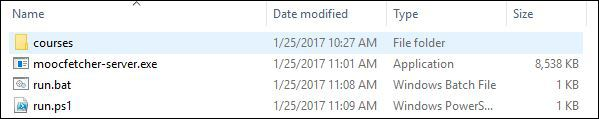
\includegraphics{moocfroot.jpg}
\caption{Directory listing containing MOOCFetcher Kiosk related files
\label{moocfroot}}
\end{figure}

\subsection{Downloading and Installing Latest
Release}\label{downloading-and-installing-latest-release}

Open your web browser and navigate to the MOOCFetcher Kiosk releases
page:

\textbf{\url{https://github.com/MOOCFetcher/moocfetcher-appliance/releases}}

You should see a page like in Figure \ref{releases}. Download the file
\textbf{moocfetcher.zip}, and extract the contents into the hard drive
containing the MOOCs.

\begin{figure}
\centering
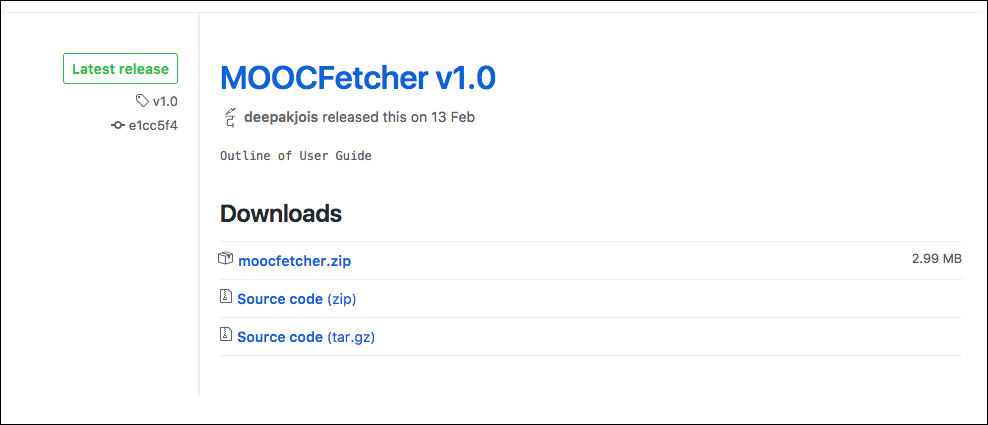
\includegraphics{releases.jpg}
\caption{MOOCFetcher Kiosk Releases Page on Github \label{releases}}
\end{figure}

\section{Using MOOCFetcher Kiosk}\label{using-moocfetcher-kiosk}

\subsubsection{Launching the MOOCFetcher Kiosk
application}\label{launching-the-moocfetcher-kiosk-application}

Navigate to the top level folder of the hard disk containing the MOOCs
in File Explorer, and then double-click the file \textbf{run.bat}. This
should launch the MOOCFetcher Kiosk application in a new window, as
shown in Figure \ref{launch}.

\begin{figure}
\centering
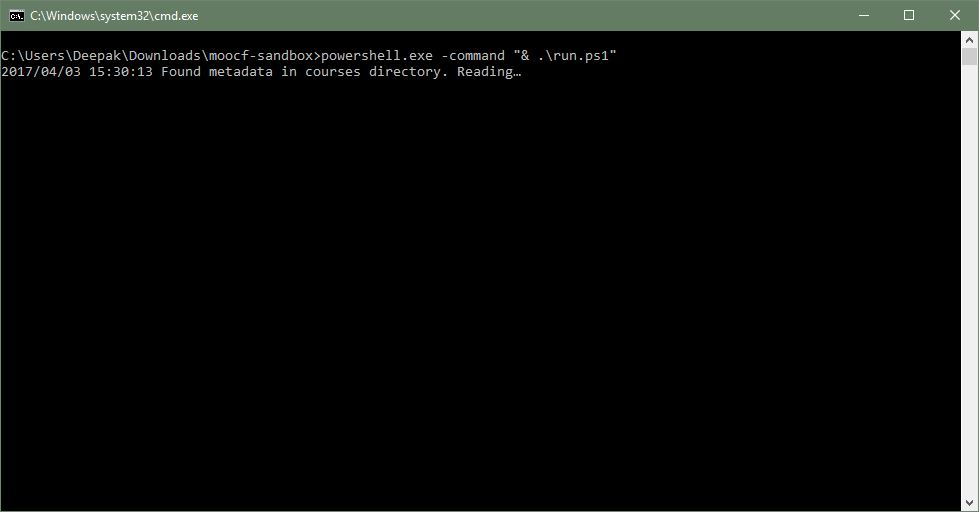
\includegraphics{launch.jpg}
\caption{MOOCFetcher Kiosk Application Launch \label{launch}}
\end{figure}

\subsection{Opening the start page in Google
Chrome}\label{opening-the-start-page-in-google-chrome}

Open the Chrome web browser, and navigate to the following location:
\textbf{http://localhost:8080}.

You should see a screen like in Figure \ref{startpage}.

\begin{figure}
\centering
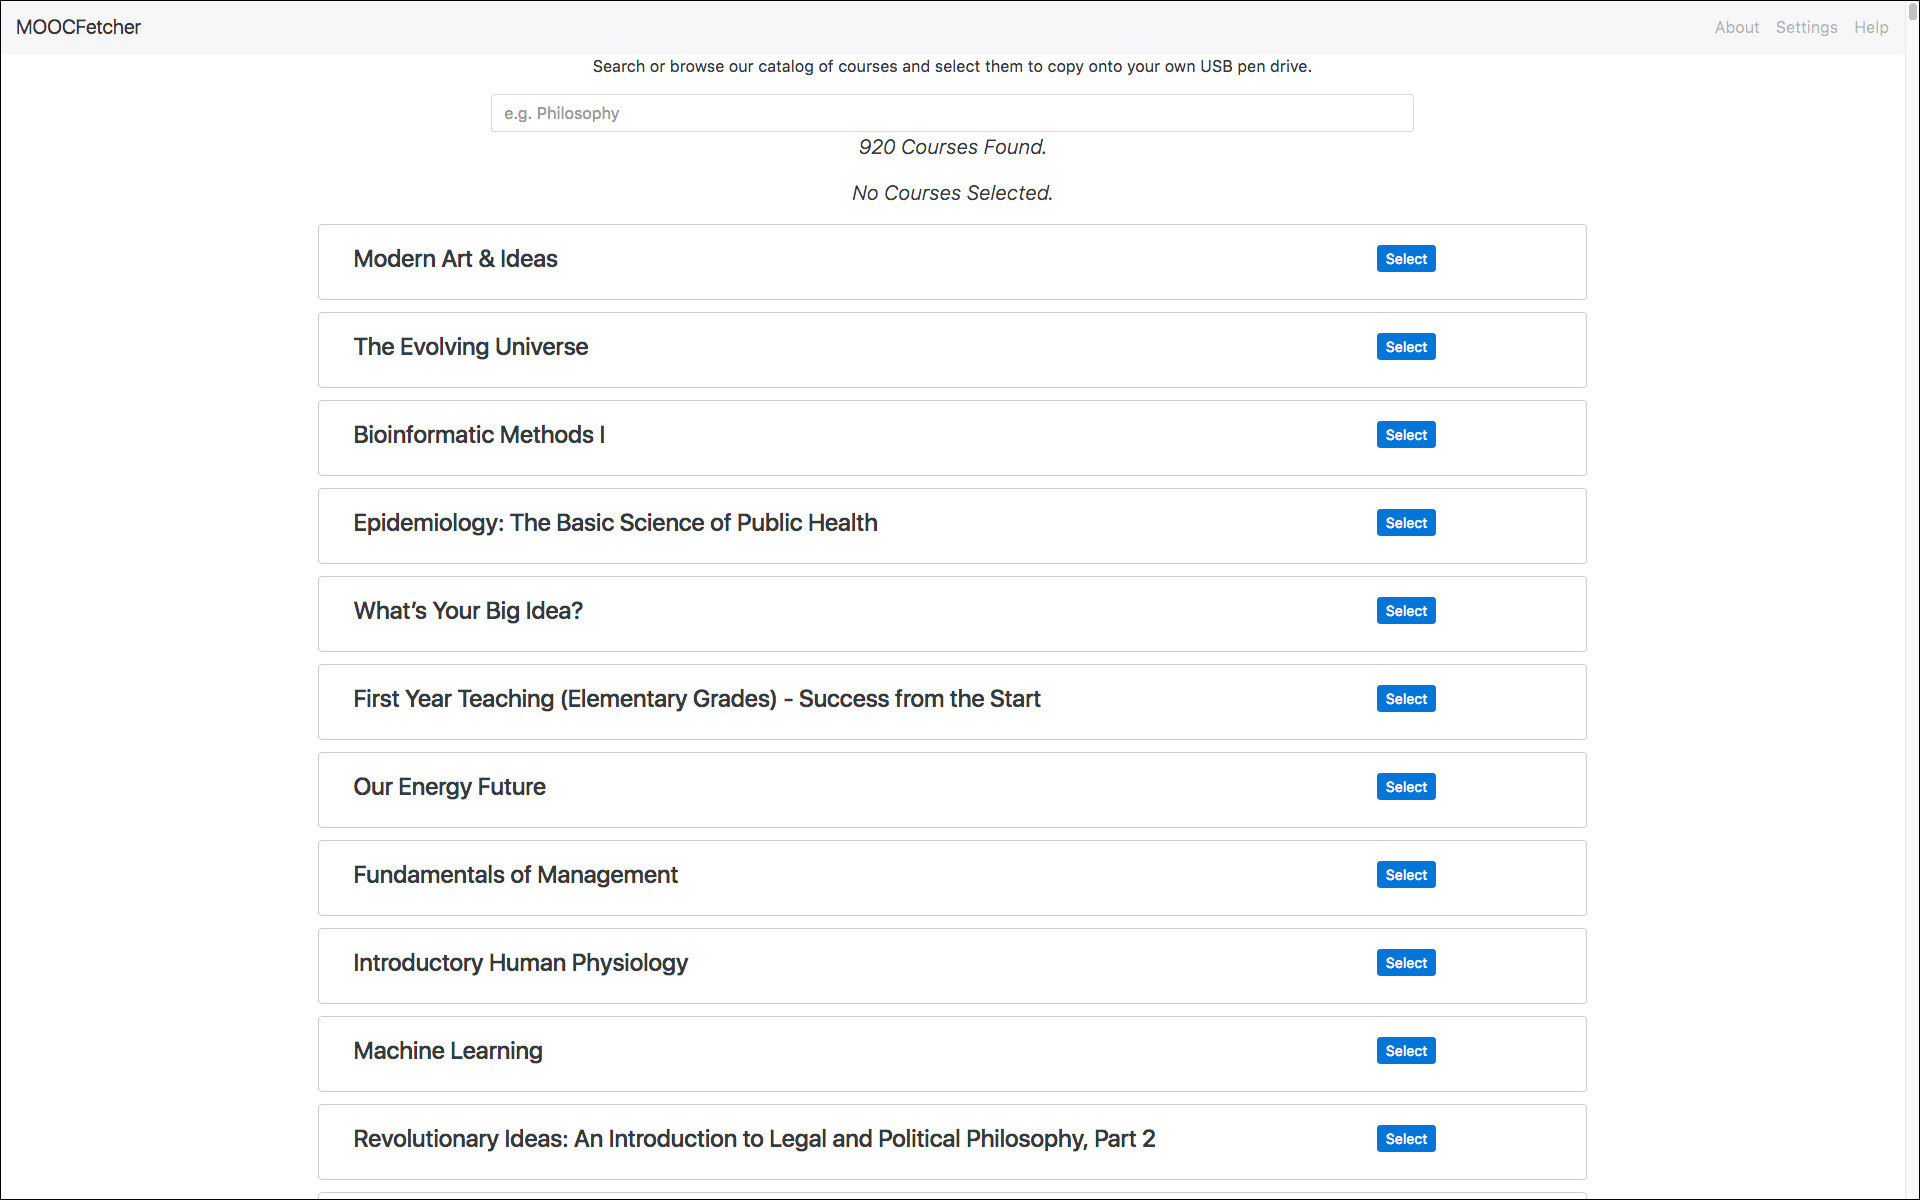
\includegraphics{step1.jpg}
\caption{MOOCFetcher Kiosk Start Page \label{startpage}}
\end{figure}

\section{Troubleshooting and
Questions}\label{troubleshooting-and-questions}

If you encounter any problems following the instructions, or have any
further questions, please e-mail us at
\textbf{\href{mailto:contact@moocfetcher.com}{\nolinkurl{contact@moocfetcher.com}}}.

\end{document}
